\documentclass[tikz, border=1cm]{standalone}
\usepackage{ifthen}

\begin{document}
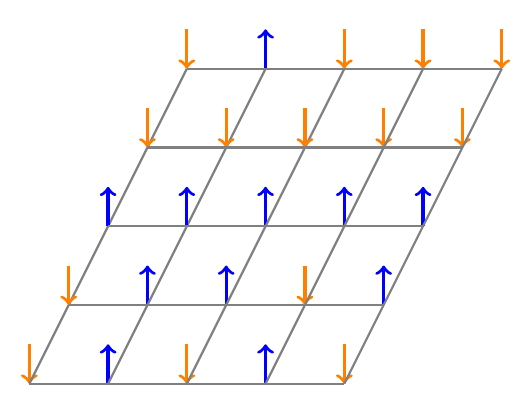
\begin{tikzpicture}
  \def\Size{5}
  \def\Ang{0.5}
    \foreach \X in {1,...,\Size} {
        \foreach \Y in {1,...,\Size} {
            \pgfmathparse{rand>0?"blue":"orange"}
            \definecolor{tempcolor}{named}{\pgfmathresult}
            \ifthenelse{\equal{\pgfmathresult}{blue}}{
                \draw[->, very thick, blue] (\Y+0.5*\X-1,\X) -- ++(0,0.5);
            }{
                \draw[<-, very thick, orange]  (\Y+0.5*\X-1,\X) -- ++(0,0.5);
            }
        }
        \draw[thick,gray] (\X*\Ang,\X) -- (\Size-1+\Ang*\X,\X);
        \draw[thick,gray] (\Ang+\X-1,1) -- (\Ang*\Size+\X-1,\Size);
    }
\end{tikzpicture}
\end{document}
